\documentclass[acmtog]{acmart}
% \documentclass[manuscript]{acmart}
\usepackage{listings}

\ExplSyntaxOn
\cs_new:Npn \ttbreakable {
  \ttfamily
  \char_set_catcode_active:N _
  \char_set_catcode_active:N .
  \char_set_catcode_active:N /
  \char_set_catcode_active:N -
  \char_set_catcode_active:N :
  \char_set_active_eq:NN _ \scan_stop:
  \char_set_active_eq:NN . \scan_stop:
  \char_set_active_eq:NN / \scan_stop:
  \char_set_active_eq:NN - \scan_stop:
  \char_set_active_eq:NN : \scan_stop:
}
\ExplSyntaxOff

%%
%% \BibTeX command to typeset BibTeX logo in the docs
\AtBeginDocument{%
  \providecommand\BibTeX{{%
    Bib\TeX}}}

%% Rights management information.  This information is sent to you
%% when you complete the rights form.  These commands have SAMPLE
%% values in them; it is your responsibility as an author to replace
%% the commands and values with those provided to you when you
%% complete the rights form.
\setcopyright{acmlicensed}
\copyrightyear{2025}
\acmYear{2025}
%\acmDOI{XXXXXXX.XXXXXXX}

%%
%% These commands are for a JOURNAL article.
%\acmJournal{TOG}
%\acmVolume{37}
%\acmNumber{4}
%\acmArticle{111}
%\acmMonth{8}

%%
%% The majority of ACM publications use numbered citations and
%% references.  The command \citestyle{authoryear} switches to the
%% "author year" style.
%%
%% If you are preparing content for an event
%% sponsored by ACM SIGGRAPH, you must use the "author year" style of
%% citations and references.
\citestyle{acmauthoryear}


%%
%% end of the preamble, start of the body of the document source.
\begin{document}

\title{Building a RAG as a Natural Way to Find Similar Patients}

\author{Seth Schwiethale}
\email{seth.schwiethale@utexas.edu}
\affiliation{%
  \institution{University of Texas at Austin}
  \city{Austin}
  \state{Texas}
  \country{USA}
}

\begin{abstract}
  Clinical notes contain rich data, but it is unstructured and difficult to query. Existing search strategies are either too rigid, requiring a specific query format, or too general, returning values with poor contextual relevance. This paper explores the utilization of a Large Language Model (LLM) via a Retrieval-Augmented Generation (RAG) system to allow a user to query the database for patients similar to a given patient using a natural language query.  We discuss the use of a hybrid retrieval routing strategy to determine an effective retrieval search space. We create multi-modal patient vectors by combining structured features (tabular data) with embeddings of the patient's discharge summary notes (unstructured text), using a clinical BERT model to embed the query and the patient notes in a GPU-accelerated environment (utilizing the NVIDIA DGX Spark), and a cosine distance metric to find the nearest neighbors. We then use the LLM to generate a response to the query, providing a clinical explanation of why the returned patients are good matches for the query. The resulting system shows promise for improving the ergonomics of clinical patient search, but requires further refinement to ensure meaningful results are consistently returned.
\end{abstract}

\keywords{Machine Learning, Natural Language Processing, RAG, Healthcare}

\received{8 December 2025}

\lstset{
    basicstyle=\fontfamily{zi4}\selectfont\small,
    breaklines=true,
    breakatwhitespace=true,
    columns=fullflexible
}

%%
%% This command processes the author and affiliation and title
%% information and builds the first part of the formatted document.
\maketitle

\section{Introduction}
When assessing a patient, clinicians draw on their experience and knowledge of previous patients. They develop intuitions based on experience and memory to guide their decision-making. Today, this direct experience can be supplemented by access to broad sources of information, but the interface to sources requires distinct, rigid and unintuitive skills, such as querying a database, using a proprietary reference tool, or interpreting complex statistical analyses. The goal of this project is to explore the use of recent developments in machine learning, specifically the use of Large Language Models (LLMs) via a Retrieval-Augmented Generation (RAG) system, to provide a more natural interface to these resources. We want to provide a tool that extends a clinician's clinical expertise to the best available evidence by the same intuitive means they use to draw upon their own clinical experience, by allowing them to ask questions like "how is this patient similar to those I have seen in the past?"

As an attempt to address these challenges, we present a hybrid RAG system for clinical case retrieval. Our specific contributions are as follows:

\begin{itemize}
  \item A RAG application applied to a multi-modal patient representation that combines structured features and unstructured text from the MIMIC-III database.
  \item A hybrid retrieval routing strategy that leverages the combination of an embedding BERT model, LLM and database filtering to facilitate a natural interface to the database.
  \item A scalable implementation, built with the NVIDIA DGX Spark, to perform the embedding generation in a GPU-accelerated environment.
\end{itemize}

\section{Related Work}
Prior work relevant to our project covers three fundamental areas: RAG frameworks, clinical-specific embedding models, and the geometry of multi-modal representation for retrieval. RAG frameworks motivate our use of retrieval to provide context to the LLM responses in patient-level evidence, while Clinical BERT models provide clinically meaningful embeddings of both discharge summaries and queries. Finally, recent work on the modality gap provides insight into the limitations of simple multi-modal retrieval and motivates design iterations in our retrieval strategy, even beyond the scope of this paper.

\subsection{Retrieval-Augmented Generation for Knowledge-Intensive NLP Tasks}

This is the seminal paper introducing the concept of Retrieval-Augmented Generation (RAG). In this method, a corpus of text is retrieved and provided as context to the LLM to help it generate a response. They demonstrate that this approach can improve the accuracy of knowledge-intensive NLP tasks, when compared to standard LLMs. \cite{lewis2020rag} We are leveraging this general approach in our project to help give the LLM patients that are similar before asking it to generate an analysis.

\subsection{Publicly Available Clinical BERT Embeddings}
The authors created publicly available BERT-based embedding models trained specifically on clinical text. They showed empirically that these domain-specific models gain substantial performance improvements on clinically-relevant tasks. We are using the Clinical BERT model \cite{alsentzer2019clinicalbert} in our paper to embed the discharge summary notes and the queries provided by the user.

\subsection{Mind the Gap: Understanding the Modality Gap in Multi-modal Contrastive Representation Learning}
This paper offers a three part explanation of how the combination of embeddings from different data types (e.g., unstructured text, tabular data) are misaligned in vector space, ending up consisting of two clusters, one for each modality \cite{liang2022modalitygap}. We are using this understanding to guide critical design decisions in the retrieval stage, including the use of a hybrid retrieval strategy.

\section{Methodology}
To build a system capable of usefully answering open-ended queries about patients similarity, we gradually transform raw MIMIC-III data into a multimodal search space usable by an LLM. We ingest and clean structured and unstructured data, engineer a subset of interpretable features, and embed clinical notes through clinical BERT, generating patient-level representations on the DGX Spark. The retrieval mechanism adapts to the user{’}s query through an LLM router. These steps together form a RAG pipeline that supports patient retrieval with a generative clinical explanation.

\begin{figure}[hbpt]
  \centering
  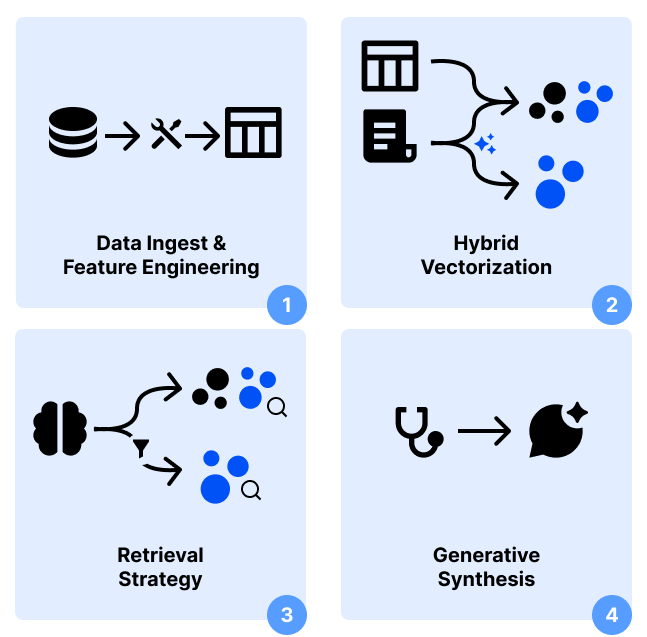
\includegraphics[width=\linewidth]{./methodology-figure.png}
  \caption{The methodology in 4 stages.}
  \label{fig:methodology}
\end{figure}

\subsection{Data Ingestion \& Feature Engineering}

We started with the structured part of the patient representation by importing and merging the \texttt{PATIENTS} with \texttt{ADMISSIONS} tables on \texttt{SUBJECT\_ID} resulting in an entry for each admission that included basic patient demographic information found in the \texttt{PATIENTS} table: \texttt{GENDER} and \texttt{DOB}. From the Admissions table, the \texttt{ETHNICITY}, \texttt{INSURANCE}, \texttt{LANGUAGE}, \texttt{RELIGION}, \texttt{MARITAL\_STATUS} columns were chosen as demographic features. From the \texttt{table DIAGNOSES\_ICD} table, we imported \texttt{ICD9\_CODE} for later use.

To prepare the unstructured Discharge summary notes for embedding, the \texttt{NOTEEVENTS} table was loaded by chunks with \texttt{pandas} \cite{pandas_docs} and only rows with \texttt{CATEGORY} equal to "Discharge summary" were kept.

Processing was necessary for the structured features to prepare them for the hybrid patient representation, where we grouped everything by \texttt{SUBJECT\_ID} to create one vector per patient (combining their notes with the structured data).

\subsubsection{The Age Calculation}

The MIMIC-III database provides the date of birth (with some caveats) from the \texttt{PATIENTS} table and the admission time from the \texttt{ADMISSIONS} table. Each patient's date of birth was subtracted from their first admission time to produce a derived  "age in" column, and then the date of birth was subtracted from their last admission to produce a derived "age out" column. Age columns are more easily scalable features for the target dataset.

\subsubsection{The Categorical Data}

The other features: {\ttfamily ETHNICITY, INSURANCE, LANGUAGE, RELIGION, MARITAL\_STATUS, GENDER, and ICD9\_CODE} are categorical values needed to be turned into numbers. 

\bigskip

Before encoding, missing values were handled as follows:
\begin{itemize}
    \item \texttt{LANGUAGE} - Because the origin of this data is the United States, it was assumed that a missing language value indicated a non-noteworthy value of "English"
    \item \texttt{MARITAL\_STATUS} - Missing values were filled with "Unknown"
    \item \texttt{RELIGION} - Missing values were filled with "Not Specified"
\end{itemize}
All other values were non-null.

\bigskip

Instead of assigning each unique value an integer value - which might skew our patient search to associate two adjacent encodings (e.g. $Married = 1, Single = 2, ... Life Partner = 7$) when no such association is warranted - we used one-hot encoding \cite{kaggle_one_hot_rutecki} to spread each unique value into a new column. If a patient's \texttt{MARITAL\_STATUS} value is "SINGLE", there is a $1$ for the value of the \texttt{SINGLE} column and a $0$ for each of the others.

\bigskip

The \texttt{RELIGION} values were slightly simplified by collapsing all denominations of Christianity into a single "Christian" value. This traded some granularity in religious affiliation with the benefit of reducing the vector dimension impact of one-hot encoding, condensing twelve columns to one.

\bigskip

For the last step in processing the structured features, the numerical columns were scaled to be between $0$ and $1$ to prevent the embeddings from having a dominating effect on the model.

\subsubsection{Reducing Dimensionality of Diagnoses}

Dimensionality was a particular concern when handling the \texttt{DIAGNOSES\_ICD} table. There are $6984$ unique diagnoses in the \texttt{DIAGNOSES\_ICD} table of the possible $14,000+$ defined ICD9 Codes; if we were to one-hot encode the values as-is, our patient vectors would be too large and very sparse (mostly zeros). Before adding diagnoses to our patient vector, the size per row was currently sitting at $146$, so we looked for a way to avoid increasing the dimensions by an order of magnitude. For our purpose, we decided that it made sense to group the codes. For example, we collapsed "Type 1 Diabetes," "Type 2 Diabetes," and "Diabetes with Complications" into a single feature: "Diabetes." To achieve this, we utilized the Clinical Classifications Software (CCS) for ICD-9-CM, which collapses the $14,000$ ICD9 Codes ``into a smaller number of clinically meaningful categories that are sometimes more useful for presenting descriptive statistics than are individual ICD-9-CM codes`` \cite{hcup_ccs}. We merged the \texttt{DIAGNOSES\_ICD} table with the CCS crosswalk on the \texttt{ICD9\_CODE} column and filled missing values with "UNMAPPED" for the \texttt{CCS\_CATEGORY}. This reduced the number of unique diagnoses from $6984$ to $281$, dramatically reducing the dimensional impact of the feature.

\subsection{Hybrid Vectorization}
In the next stage, we combined the structured features with embeddings of discharge summary notes, made with the clinical BERT model  \cite{bioclinicalbert}, into a single vector for each patient.

\subsubsection{NVIDIA DGX Spark}
We had remote access to a NVIDIA DGX Spark \cite{dgx_spark} machine, which was used to perform the embedding generation in a GPU-accelerated environment. Being a recently-released platform, not all libraries were available in the standard Python environment, so to use \texttt{pytorch} \cite{pytorch_website} and `transformers` \cite{huggingface_transformers_docs} with access to the $6,144$ CUDA cores we ran our code in the NVIDIA-provided PyTorch docker image \cite{dgx_spark_docker_image} on the Spark to perform the embedding generation. The same environment was later used to run the retrieval and generative synthesis stages.

\subsubsection{Clinical BERT Embeddings}
We embedded discharge summaries only. The \texttt{NOTEEVENTS} table was streamed in 10{,}000 row chunks with \texttt{pandas}, filtered by \texttt{CATEGORY == "Discharge summary"}, and then grouped by \texttt{SUBJECT\_ID}, concatenating each patient’s summaries into one string separated by delimiters. We used Clinical BERT  via \texttt{transformers} and PyTorch, tokenizing with \texttt{max\_length=512} and an overlapping stride of $100$ to handle long notes. We iterated over patients, batched on GPU, collected embeddings and subject IDs, then aggregated the individual summary representations of multiple text chunks into a single, comprehensive vector that represents the entire set discharge summaries for a patient. Finally, we saved them to file for use in the downstream retrieval and generative synthesis stages. It took roughly 1 hour to embed the discharge summaries for all of the patients on the DGX Spark.

\bigskip

Our final patient vector consisted of our $426$-dimension structured features plus the $768$-dimensional vector from the clinical BERT embeddings. Our hypbrid patient representation had $41{,}117$ patients, each with a combined vector dimension of $1{,}194$.


\subsection{Retrieval Strategy}
With the patient vectors in their multimodal format, we are able to perform patient-to-patient similarity searches. Given one patient's vector, we could find the $k$ nearest neighbors in the patient space. We used the \texttt{sklearn} library \cite{scikitlearn_neighbors_docs} to perform the nearest neighbor search with the cosine distance metric.


\begin{verbatim}
Patients similar to 19:
  Match #1: Patient 19835 (Similarity: 76.3%)
  Match #2: Patient 3340 (Similarity: 71.5%)
  Match #3: Patient 60423 (Similarity: 71.4%)
  Match #4: Patient 29813 (Similarity: 68.4%)
  Match #5: Patient 1909 (Similarity: 68.3%)
\end{verbatim}

For the authors, this was the stage where their understanding of the RAG pipeline and the retrieval strategy became more concrete. The goal of this project was to allow a user to intuitively query the database for patients similar to a given patient; we want to avoid forcing the user to use a specific query format, but so far we had only a system that accpeted an explicit subject ID. If found, we used that patient's vector to search for nearest neighbors. For use cases like "Find patients similar to patient 19", this worked well, but for any query more complex than that, it was clear that we needed to use a more sophisticated approach.

\subsubsection{Learning about the Modality Gap the Hard Way}

We quickly discovered that there is a well-known challenge referred to as the "Modality Gap" \cite{liang2022modalitygap}, where embeddings from different data types (e.g., unstructured text, tabular data) are misaligned in vector space. We had spent a significant extent of our Feature Engineering efforts to create a hybrid patient representation that combined the structured (tabular) features with the embeddings of the discharge summaries (unstructured text).

But the initial implementation of our patient retrieval simply embedded the query with the clinical BERT embedding model and produced a $768$-dimension vector. So, we could not actually effectively utilize the extra $426$-dimensions we had added from the structured features. The query embedding was suited only for searching the space of the discharge summary embeddings; padding the query embeddings with zeros would introduce a large amount of noise. We wanted a tool that could leverage the tabular data as well as the text data, since the structured data had important signals that we expected to be useful for the retrieval process.

\subsubsection{Creating a Router}
It became clear that our retrieval strategy would need to be made modular, so it could handle choosing an appropriate search strategy based on the query. We decided to incorporate the LLM as a prestep to the retrieval process, to handle the query in a more flexible way. We effectively used the LLM as a routing layer, to guide the retrieval process based on the intent of the query. 

This, we discovered, is not an exact science; designing a robust router presented significant challenges in prompt engineering and intent classification. In evaluating our RAG we continue to find cases where either the LLM makes mistakes extracting the parameters we want or we aren't supporting intuitive use cases. Frankly, this is the piece we have continued to try to revise up until the final submission of this report. Further research, both in the field of Usability Design and in the domain of existing work on RAG systems, would be required to create an ideal router, one that could interpret the query and determine the most effective way to search the dataset, but we set out to establish a baseline that could be used to create a more sophisticated router in the future.

Our modular approach first classifies user intent based on the query. If the query includes a subject ID, we treat the query as a specific user lookup and use the multimodal patient vector to search for nearest neighbors. If the query does not include a subject ID, we extract structured parameters from the query. For any features found in the query, the search space is filtered to only include patients that match the query parameters. To accomplish the search space filtering, we wrote a function that forms a prompt for the LLM, directing it to extract a set of parameters from the query and return them in JSON format.

\begin{lstlisting}
  Extract structured filters from this patient search query. Return ONLY valid JSON.

  Query: "{query}"

  Available diagnosis categories (examples): {diagnoses_context}

  Return JSON with these fields (use null for missing values):
{{
    "gender": "M" or "F" or null,
    "age_min": integer or null,
    "age_max": integer or null,  
    "ethnicity": string or null (ONLY race/ethnic background like "WHITE", "BLACK/AFRICAN AMERICAN", "ASIAN - CHINESE"),
    "religion": string or null (religious affiliation like "CHRISTIAN", "JEWISH", "MUSLIM", "BUDDHIST", "NOT SPECIFIED"),
    "diagnoses": [list of diagnosis category names that match the query] or []
}}
  ... # truncated
\end{lstlisting}

Once the router has identified the search space most appropriate to address the query's intent, we embed the query and search the filtered space using only the embeddings from the discharge summaries. These queries would not be able to utilize the multimodal patient representations, but by reducing their search space we attempted to improve the chances of finding relevant result.

\subsection{Generative Synthesis}
The final stage in our RAG pipeline involved feeding the Discharge Summary of the patients found in the retrieval stage to the LLM to generate a response to the query, providing a clinical explanation of why the returned patients are good matches for the query. The goal is to synthesize clinical details scattered throughout the notes text into a coherent answer, rather than just return a wall of text.

Here, the LLM choice dictates constraints on the parameters used, including the context window length. Because the notes can be quite long and we were using the Mistral 7B model, we set a conservative context window length to ~22{,}000 words, based on the model's documentation \cite{obot_mistral7b_instruct}.

Because we used the DGX Spark, we had access to a large amount of memory and decided to opt for percision of performance by not using 4-bit quantization.

For the answer prompts, we provided a system role to guide the LLM's response, providing a clinical explanation of why the returned patients are good matches for the query.

\begin{quote}
  "role": "system", 
  "content": "You are an expert medical AI. Answer based ONLY on the provided patient history. Be concise and clinically relevant. Provide insights into why the provided PATIENT HISTORY is a good match for the QUESTION."

\end{quote}

The prompt in the user role contained the (potentially truncated) Discharge Summary of the patients found in the retrieval stage and the query.

\begin{lstlisting}
  "role": "user", 
  "content": "--- PATIENT HISTORY ---\n<notes>\n\nQUESTION: <query>"
\end{lstlisting}

\section{Results}

TODO: discuss tuning context window for discharge notes to address "Lost in the Middle" problem. Look more into The "Needle in a Haystack" Test

\section{Conclusion}

\bibliographystyle{ACM-Reference-Format}
\bibliography{references}

\end{document}
\endinput
%%
%% End of file `sample-acmtog.tex'.
